\documentclass{article}
\usepackage{v-test-paper}
\title{\textsc{Vectors}}
\date{February 21, 2024}

\newcommand{\itemstared}{\refstepcounter{enumi}\item[$^\star$\theenumi.]}
\usetikzlibrary{matrix,  positioning, patterns, backgrounds}
\renewcommand{\ans}{\quad}


\tikzstyle{root} = [rectangle, rounded corners, 
minimum width=3cm, 
minimum height=0.7cm,
text centered, 
draw, 
font=\scshape,
]
\tikzstyle{child} = [rectangle, rounded corners, 
inner sep=2mm,
text centered, 
draw, 
font=\itshape,
text width=3.25cm,
]

\tikzstyle{child-branch} = [rectangle, rounded corners, 
inner sep=2mm,
text centered, 
draw, 
font=\itshape,
text width=2.5cm,
level distance=5mm,
]



\tikzstyle{arrow} = [thick,->,>=latex]



\begin{document}
\maketitle
\begin{center}
\begin{tikzpicture}[node distance=2cm]

\matrix [column sep=10mm,row sep=10mm]
{
&\node (root) [root] {Vectors};\\
\node (child-left)[child] {Definition of Vectors}; & 
\node (child-center)[child] {Addition of Vectors}; &
\node (child-right)[child] {Multiplication of Vectors}; \\
\node (child-left-b)[child] {Geometrical Interpretation}; &
\node (child-center-b)[child] {Triangle and Parallelogram Law and their equivalence}; &
\node[child-branch](child-right-bl)at ($(child-right.south)+(-1.5, 0.5)$){Dot Product};
\node[child-branch](child-right-br)at ($(child-right.south)+(+1.5, 0.5)$){Cross Product};\\
\node (child-left-bb)[child] {Additive inverse of a Vector}; &
\node (child-center-bb)[child]{Resolution of Vectors in two perpendicular components};&
\node[child-branch](child-right-blb)at ($(child-right-bl.south)+(0, 0.5)$){Projection of Vector};
\node[child-branch](child-right-brb)at ($(child-right-br.south)+(0, 0.5)$){Cross Product as area};\\
\node(child-left-bbb)[child]{Scalar Multiplication of a Vecctor};\\
};

\draw [arrow] (root) -| (child-left);
\draw [arrow] (root) -- (child-center);
\draw [arrow] (root) -| (child-right);
\draw [arrow] (child-left) --(child-left-b);
\draw [arrow] (child-center) --(child-center-b);
\draw [arrow] (child-right) -- (child-right-bl);
\draw [arrow] (child-right) -- (child-right-br);
\draw [arrow] (child-left-b)--(child-left-bb);
\draw [arrow] (child-left-bb)--(child-left-bbb);
\draw [arrow] (child-center-b)--(child-center-bb);
\draw[arrow] (child-right-bl)--(child-right-blb);
\draw[arrow] (child-right-br)--(child-right-brb);
\end{tikzpicture}
\end{center}


\begin{multicols}{2}
\begin{flushleft}
\begin{align*}
    |\vec{a}+\vec{b}| &= \sqrt{a^2+b^2+2ab \cos \theta}\\
    |\vec{a}+\vec{b}|_{\textit{max}} &= a+b \hspace{5 mm} \text{when}~ \theta=0^\circ \\
    |\vec{a}+\vec{b}|_{\textit{min}} &= |a-b| \hspace{3.5 mm} \text{when}~ \theta=180^\circ \\
     \tan \alpha &=\dfrac{b\sin \theta}{a+b\cos \theta}
    \end{align*}
\end{flushleft}
\begin{flushright}
    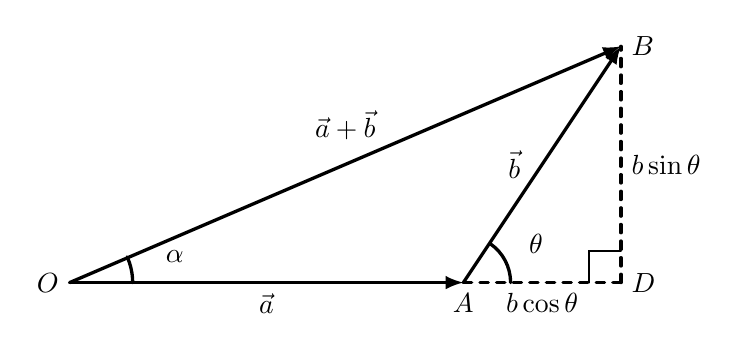
\begin{tikzpicture}[cap=round, very thick, >=latex]
        \draw[->](0, 0)node[below, left]{$O$}--(5, 0) node[below, midway]{$\vec{a}$};
        \draw[dashed](5, 0)node[below]{$A$}--(7, 0) node[below, right]{$D$} node[below, midway]{$b\cos\theta$};
        \draw[dashed](7, 0)--(7, 3) node[below, right]{$B$} node[right, midway]{$b\sin\theta$};
        \draw[thick](6.6, 0)--(6.6, 0.4)--(7, 0.4);
        \draw[->](5, 0)--(7, 3)node[midway, left=4pt]{$\vec{b}$};
        \draw[->](0, 0)--(7, 3)node[midway, above=5pt]{$\vec{a}+\vec{b}$};
        \draw (0.8, 0) arc[start angle=0, end angle=24, radius=0.8] node[right=10pt]{$\alpha$};
        \draw (5.6, 0) arc[start angle=0, end angle=55, radius=0.6] node[right=10pt]{$\theta$};
    \end{tikzpicture}
\end{flushright}
\end{multicols}

\begin{multicols}{2}
    \begin{flushleft}
        \begin{enumerate}
            \item[.] Properties of Scalar Triple Product
                \begin{itemize}
                \item $\vec{a} \cdot (\vec{b} \times \vec{c}) = (\vec{a} \times \vec{b}) \cdot \vec{c}$
                \item $\vec{a} \cdot (\vec{b} \times \vec{c}) = \vec{b} \cdot (\vec{c} \times \vec{a}) = \vec{c} \cdot (\vec{a} \times \vec{b})$
                \item $\vec{a} \cdot (\vec{b} \times \vec{c}) = [\vec{a} \vec{b} \vec{c}] = 0$ \\if and only if $\vec{a}$, $\vec{b}$~and~$\vec{c}$ are coplanar.
                \end{itemize}
        \end{enumerate}
    \end{flushleft}
    \begin{flushright}
        \begin{enumerate}
            \item[.] Properties of Vector Triple Product
                \begin{itemize}
                \item $\vec{a} \times (\vec{b} \times \vec{c}) \neq (\vec{a} \times \vec{b}) \times \vec{c}$
                \item $\vec{a} \times (\vec{b} \times \vec{c}) = (\vec{a} \cdot \vec{c}) \vec{b} - (\vec{a} \cdot \vec{b})  \vec{c}$
                \item $(\vec{a} \times \vec{b}) \times \vec{c} = (\vec{a} \cdot \vec{c})\vec{b}-(\vec{b} \cdot \vec{c})\vec{a}$
                \end{itemize}
        \end{enumerate}
    \end{flushright}
\end{multicols}

\begin{multicols}{2}
    \begin{flushleft}
        \begin{align*}
            \intertext{Area of this Parallelogram can be expressed using Cross Product of Vectors $\vec{a}$ and $\vec{b}$}
            \textit{area} &= | \vec{a} \times \vec{b} |
        \end{align*}
    \end{flushleft}
    \begin{flushright}
        \begin{tikzpicture}
            \tzline[->](0, 0)(4, 0){$\vec{a}$}[mb]
            \tzline[->](0, 0)(1.5, 1.5){$\vec{b}$}[ma]
            \tzline+[dashed](1.5, 1.5)(4, 0)
            \tzline+[dashed](4, 0)(1.5, 1.5)
        \end{tikzpicture}
    \end{flushright}
\end{multicols}

\pagebreak

\begin{enumerate}
    \item A vector of magnitude $a$ is turned through angle $\theta$. The magnitude of change in the vector is given by:
        \begin{tasks}(2)
            \task $|2a\sin \theta|$
            \task $|2a\sin\dfrac{\theta}{2}|$\ans
            \task $\left|\dfrac{a}{2}\sin \theta\right| $
            \task $\left|\dfrac{a}{2}\sin \dfrac{\theta}{2}\right|$
        \end{tasks}

    \item If $\vec{A}, \vec{B}, \vec{C},$ are mutually perpendicular vectors then which of the following is wrong?
        \begin{tasks}(2)
            \task $\vec{C} \times (\vec{A} \times \vec{B})=0$
            \task $\dfrac{\vec{A} \times \vec{B}}{|\vec{A} \times \vec{B}|}=\dfrac{-\vec{C}}{|\vec{C}|}$ \ans
            \task $\vec{A} \cdot \vec{B}=\vec{B} \cdot \vec{C}=\vec{C} \cdot \vec{A}=0$
            \task $(\vec{B} + \vec{C})$ is perpendicular to $\vec{A}$
        \end{tasks}
    
    \item The adjacent sides of a parallelogram is represented by vectors $2\hat{i}+3\hat{j}$ and $\hat{i}+4\hat{j}$. The area of the parallelogram is:
        \begin{tasks}(2)
            \task $5$ units \ans
            \task $3$ units
            \task $8$ units
            \task $11$ units
        \end{tasks}

    \item The velocity of a particle varies with time as per the law $\vec{V}=\vec{a}+\vec{b}t $ where $\vec{a}$ and $\vec{b}$ are two constant vectors. The time at which velocity of the particle is perpendicular to the velocity of the particle at $t=0$ is:
        \begin{tasks}(2)
        \task $-\dfrac{|\vec{a}|}{\vec{a} \cdot \vec{b}}$
        \task $-\dfrac{|\vec{a}|^2}{\vec{a} \cdot \vec{b}}$\ans
        \task $-\dfrac{\vec{a} \cdot \vec{b}}{|\vec{a}|^2}$
        \task None of these
        \end{tasks}	
        
        
    \item The projection of a vector $r=3\hat{i} + \hat{j} + 2\hat{k}$ on the $x-y$ plane has magnitude :
        \begin{tasks}(2)
        \task $3$
        \task $4$
        \task $\sqrt{14}$
        \task $\sqrt{10}$\ans
        \end{tasks}

    \itemstared Two particles, 1 and 2, move with constant velocities $\vec{v_1}$ and $\vec{v_2}$. At the initial moment their radius vectors are equal to $\vec{r_1}$ and $\vec{r_2}$. How must these four vectors be interrelated for the particles to collide?
        \begin{tasks}(2)
            \task $\dfrac{\vec{r_1}-\vec{r_2}}{|\vec{r_1}-\vec{r_2}|}=\dfrac{\vec{v_1}-\vec{v_2}}{|\vec{v_1}-\vec{v_2}|}$
            \task $\dfrac{\vec{r_1}-\vec{r_2}}{|\vec{r_1}-\vec{r_2}|}=\dfrac{\vec{v_2}-\vec{v_1}}{|\vec{v_2}-\vec{v_1}|}$\ans
            \task $\dfrac{\vec{r_1}-\vec{r_2}}{|\vec{v_2}-\vec{v_1}|}=\dfrac{\vec{v_2}-\vec{v_1}}{|\vec{r_1}-\vec{r_2}|}$
            \task None of these
        \end{tasks}

    \item If $\vec{a_1}$ and $\vec{a_2}$ are two non-collinear unit vector and if $|\vec{a_1} + \vec{a_2}|=\sqrt{3}$, then the value of $(\vec{a_1}-\vec{a_2})\cdot(2\vec{a_1}+\vec{a_2})$ is:
        \begin{tasks}(2)
            \task $2$
            \task $3/2$
            \task $1/2$\ans
            \task $1$
        \end{tasks}

    \item Let $\vec{c} = \vec{a} + \vec{b}$. Which of the following is (are) true?
        \begin{tasks}(2)
            \task $|a-b| \leq c \leq a+b$\ans
            \task $c$ is maximum if $\vec{a}$ and $\vec{b}$ are parallel \ans
            \task $c \geq \text{minimum} ~(a, b)$
            \task $c \leq \text{maximum}~ (a, b)$
        \end{tasks}

    \item The maximum number of components into which a vector can be resolved is
        \begin{tasks}(2)
            \task 2
            \task 3
            \task infinite \ans
            \task 4
        \end{tasks}

    \item Three forces $\vec{F_1}$, $\vec{F_2}$ and $\vec{F_3}$ act on a block. $\vec{F_1} + \vec{F_2} + \vec{F_3} = 0$ Which of the following is (are) true?
        \begin{tasks}(2)
            \task $\vec{F_1}$, $\vec{F_2}$ and $\vec{F_3}$ form the sides of a triangle \ans
            \task $F_1 + F_2 > F_3$\ans
            \task $|F_1 - F_2| < F_3$\ans
            \task ${F_1}^2 + {F_2}^2 + {F_3}^2 + 2 \vec{F_1} \cdot \vec{F_2} + 2\vec{F_2} \cdot \vec{F_3} + 2 \vec{F_3} \cdot \vec{F_1}=0$\ans
        \end{tasks}

\end{enumerate}


\pagebreak

\begin{center}
\texttt{Answer Key}
\begin{multicols}{5}
\begin{enumerate}
\item (b)
\item (a)
\item (b)
\item (c)
\item (d)
\item (a)
\item (b)
\item (c)
\item (a)
\item (a)
\item (b)
\item (a)
\item (b)
\item (a)
\end{enumerate}
\end{multicols}
\end{center}






\end{document}